\chapter{Triển khai thử nghiệm và giao diện hệ thống}

\section{Mục tiêu hiện thực hệ thống}
Tầng triển khai thử nghiệm được xây dựng nhằm minh họa khả năng vận hành của toàn bộ pipeline NLP/RAG trên môi trường local. Giao diện không thay thế cho đánh giá định lượng trong Chương 6, nhưng giúp kiểm tra luồng xử lý thực tế: nhập review để dự đoán sentiment, nhập câu hỏi để truy xuất review liên quan, hiển thị câu trả lời có citation và trình bày thông tin kỹ thuật của corpus/index.

Một nguyên tắc quan trọng trong thiết kế giao diện là tách rõ hai loại input. Review sản phẩm được gửi đến sentiment classifier. Câu hỏi RAG được gửi đến retriever và answer generator. Thiết kế này tránh hiểu nhầm rằng model sentiment đang phân tích câu hỏi như một review.

\section{Backend FastAPI}
Backend được hiện thực bằng FastAPI. FastAPI phù hợp cho thử nghiệm vì có cú pháp gọn, hỗ trợ JSON API và dễ tích hợp với frontend tĩnh \cite{fastapi}. Backend chịu trách nhiệm load model sentiment, load FAISS index/metadata, chạy retrieval và trả kết quả ở dạng JSON.

\begingroup
\small
\begin{longtable}{L{0.22\textwidth}L{0.16\textwidth}L{0.24\textwidth}L{0.28\textwidth}}
\caption{API backend của hệ thống thử nghiệm}\label{tab:backend-api}\\
\toprule
Endpoint & Phương thức & Input chính & Output chính \\
\midrule
\code{/api/health} & GET & Không có & Trạng thái backend, đường dẫn corpus và tổng số review nếu load được. \\
\code{/api/config} & GET & Không có & Cấu hình model/index, category, metric và thông tin hiển thị cho tab kỹ thuật. \\
\code{/api/sentiment} & POST & Một review sản phẩm & Nhãn sentiment dự đoán, model đang dùng và thông tin confidence/margin nếu có. \\
\code{/api/rag} & POST & Query RAG, top-k và filter & Câu trả lời có bằng chứng, danh sách evidence, query mở rộng và thông tin debug. \\
\bottomrule
\end{longtable}
\endgroup

Backend load artifact sentiment chính, bao gồm cả \TFIDF{} vectorizer và classifier. Backend cũng load FAISS index và metadata RAG. Các tài nguyên này được cache để giảm thời gian xử lý cho các request sau.

\section{Frontend}
Frontend gồm ba thành phần chính: cấu trúc HTML, style CSS và logic JavaScript. Phần HTML định nghĩa cấu trúc tab, form và panel kết quả; phần CSS định nghĩa layout, card, badge, màu sắc và responsive behavior; phần JavaScript quản lý state, gọi API backend và render câu trả lời/evidence.

Giao diện gồm ba tab. Tab “Phân tích Sentiment” cho phép nhập một review thật và nhận nhãn tiêu cực/trung lập/tích cực. Tab “Hỏi đáp RAG” cho phép đặt câu hỏi về review, xem cách hệ thống hiểu câu hỏi, xem câu trả lời có bằng chứng và các review được truy xuất. Tab “Kỹ thuật \& đánh giá” hiển thị số documents, embedding model, retrieval method, baseline Precision@5 và đường dẫn artifact.

\section{Luồng xử lý request}
Với request sentiment, frontend gửi review đến endpoint sentiment. Backend đưa review qua pipeline model tốt nhất, gồm \TFIDF{} vectorizer và Linear SVM classifier. Kết quả trả về là sentiment label và thông tin phụ trợ.

Với request RAG, frontend gửi query, top-k và filter đến endpoint RAG. Backend chuẩn hóa query, suy luận aspect/filter nếu bật chế độ tự động, mở rộng query theo rule tiếng Việt, encode query bằng E5 với prefix \code{query: }, tìm candidates trong FAISS, áp dụng filter/rerank, sau đó tạo answer dạng template-based. Answer chỉ dùng nội dung từ evidence được truy xuất, không gọi API LLM bên ngoài.

\section{Ví dụ request/response}
Ví dụ request sentiment:
\begin{lstlisting}[language=json]
{
  "text": "Shop giao sai mau, nhan tin ho tro nhung khong tra loi."
}
\end{lstlisting}
Nội dung ví dụ tương ứng với review: “Shop giao sai màu, nhắn tin hỗ trợ nhưng không trả lời.”

Ví dụ response rút gọn:
\begin{lstlisting}[language=json]
{
  "sentiment": "negative",
  "model": "TF-IDF + Linear SVM",
  "note": "Nhan duoc du doan tu noi dung review dau vao."
}
\end{lstlisting}

Ví dụ request RAG:
\begin{lstlisting}[language=json]
{
  "query": "Khach hang phan nan gi ve giao hang cham?",
  "top_k": 5,
  "sentiment": "auto",
  "category": "all"
}
\end{lstlisting}
Nội dung ví dụ tương ứng với câu hỏi: “Khách hàng phàn nàn gì về giao hàng chậm?”

Ví dụ response RAG được rút gọn để minh họa cấu trúc:
\begin{lstlisting}[language=json]
{
  "answer": {
    "summary": "Trong cac review duoc truy xuat, phan nan tap trung vao giao hang cham, xu ly don thieu nhat quan va ho tro sau ban chua tot.",
    "issues": [
      {"text": "Giao hang cham hoac xu ly don lau.", "citations": [1, 3]},
      {"text": "Co truong hop giao sai hoac thieu hang.", "citations": [2]}
    ],
    "confidence": "medium"
  },
  "evidence": [
    {"citation": 1, "rating": 1, "sentiment": "negative", "comment": "..."}
  ]
}
\end{lstlisting}

\section{Mô tả giao diện thử nghiệm}
Trong phạm vi báo cáo, giao diện được dùng như một lớp minh họa trực quan cho pipeline đã xây dựng. Ba tab giao diện tương ứng với ba mục tiêu kiểm thử: dự đoán sentiment cho một review, hỏi đáp RAG có bằng chứng và kiểm tra thông tin kỹ thuật của artifact. Các hình trong mục này không thay thế cho đánh giá định lượng ở Chương 6, mà bổ sung bằng chứng trực quan rằng các artifact của mô hình, retrieval và backend đã được kết nối thành một hệ thống thử nghiệm thống nhất.

\begingroup
\small
\begin{longtable}{L{0.22\textwidth}L{0.24\textwidth}L{0.25\textwidth}L{0.21\textwidth}}
\caption{Vai trò kiểm chứng của các tab trong giao diện thử nghiệm}\label{tab:web-demo-tabs}\\
\toprule
Tab & Input chính & Output hiển thị & Vai trò kiểm chứng \\
\midrule
Phân tích Sentiment & Một review sản phẩm tiếng Việt & Nhãn sentiment dự đoán, model đang dùng và confidence/margin & Kiểm tra khả năng load và inference của mô hình sentiment. \\
Hỏi đáp RAG & Câu hỏi về review, top-k và filter nếu có & Câu trả lời có citation, vấn đề chính và evidence cards & Kiểm tra luồng retrieval, reranking, template answer và citation. \\
Kỹ thuật \& đánh giá & Không bắt buộc & Số documents, embedding model, retrieval method, Precision@5 và đường dẫn artifact & Kiểm tra cấu hình final và metric chính của hệ thống. \\
\bottomrule
\end{longtable}
\endgroup

\section{Minh họa demo web}
Hình \ref{fig:web-sentiment-demo} minh họa tab Phân tích Sentiment. Người dùng nhập một review sản phẩm thật; hệ thống trả nhãn cảm xúc dự đoán là tiêu cực, đồng thời hiển thị artifact model đang dùng và confidence/margin. Ví dụ này xác nhận tab Sentiment chỉ nhận review làm input, không dùng để phân tích câu hỏi RAG.

\begin{figure}[H]
    \centering
    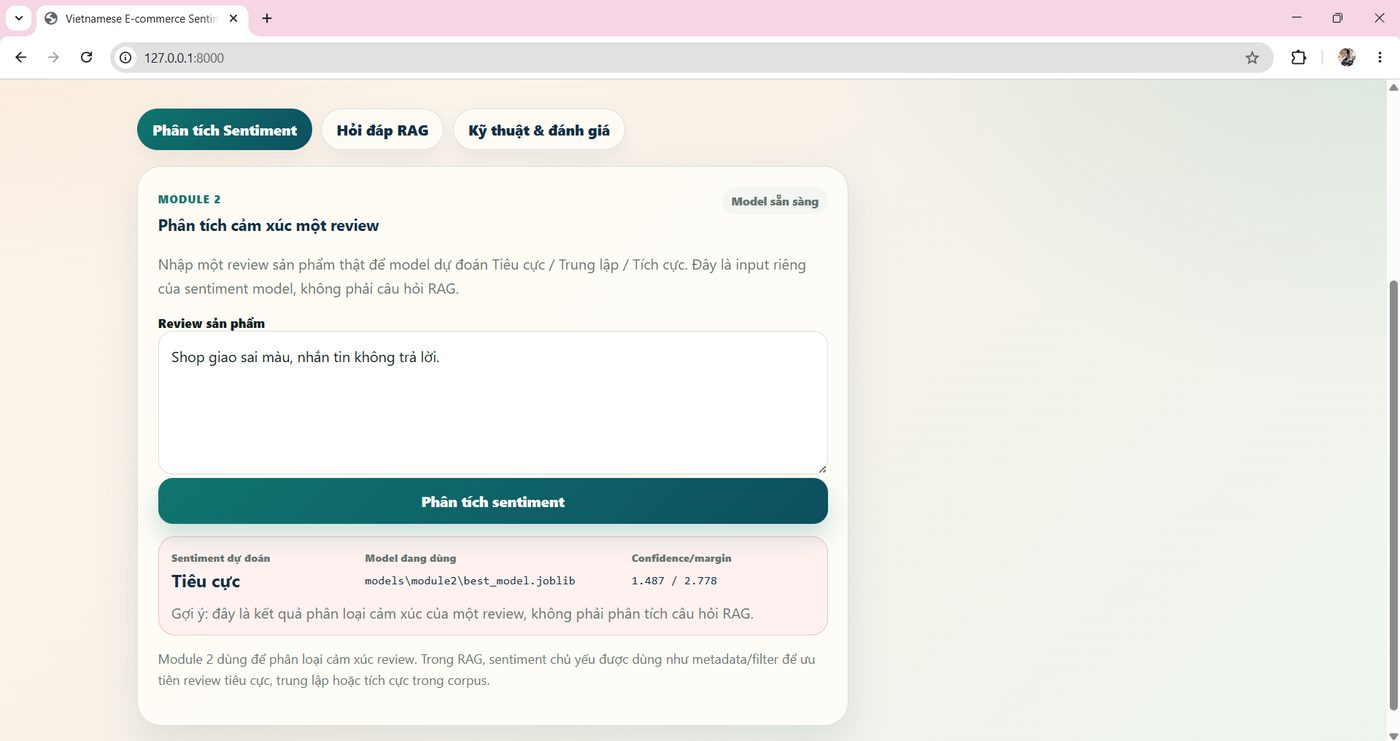
\includegraphics[width=0.92\textwidth]{figures_generated/web_sentiment_demo.jpg}
    \caption{Giao diện tab Phân tích Sentiment với ví dụ review tiêu cực.}
    \label{fig:web-sentiment-demo}
\end{figure}

Hình \ref{fig:web-rag-query-demo} thể hiện tab Hỏi đáp RAG ở bước nhập câu hỏi. Giao diện hiển thị các gợi ý truy vấn như giao hàng chậm, sai hàng, thiếu hàng, đóng gói lỗi hoặc chất lượng kém. Các gợi ý này giúp kiểm thử những nhóm complaint thường gặp trong review thương mại điện tử.

\begin{figure}[H]
    \centering
    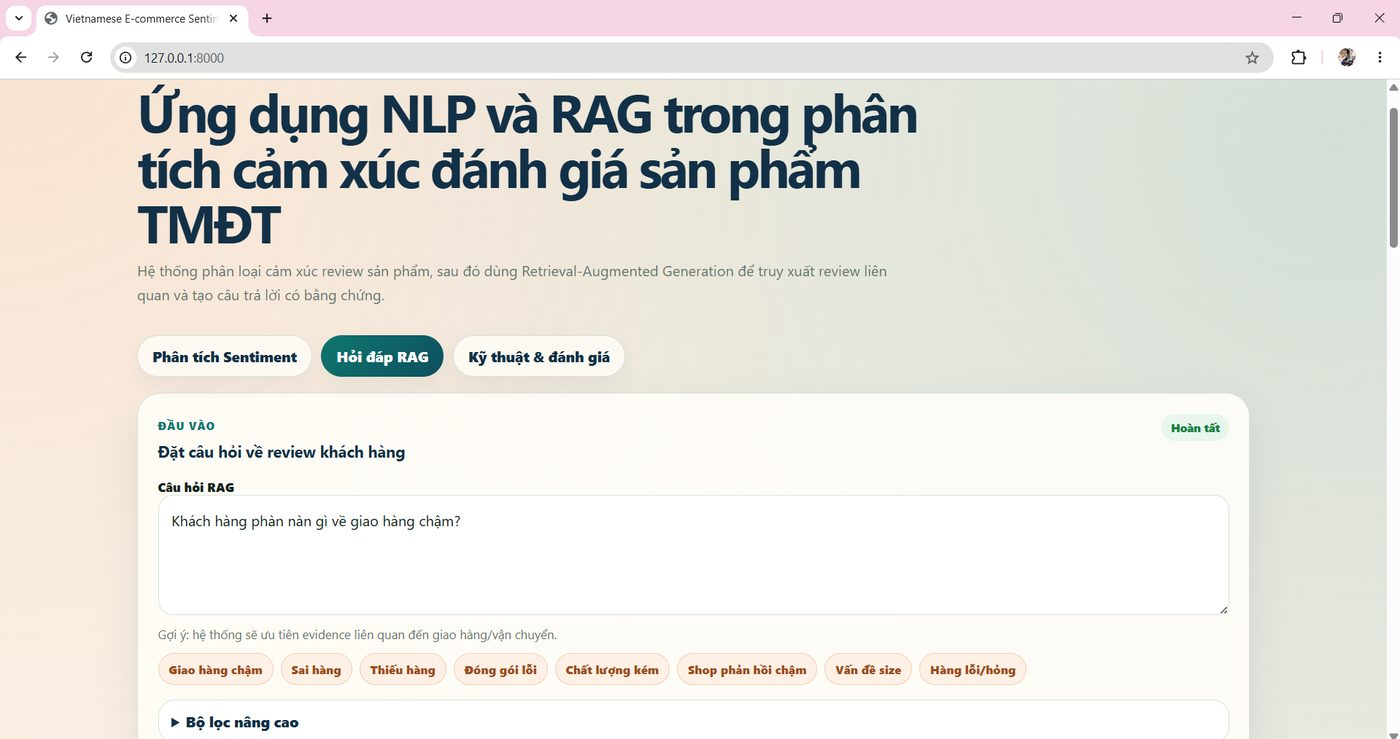
\includegraphics[width=0.92\textwidth]{figures_generated/web_rag_query_demo.jpg}
    \caption{Giao diện tab Hỏi đáp RAG ở bước nhập câu hỏi về review khách hàng.}
    \label{fig:web-rag-query-demo}
\end{figure}

\clearpage

Hình \ref{fig:web-rag-answer-demo} minh họa kết quả RAG sau khi thực thi truy vấn. Câu trả lời được trình bày theo hướng \EvidenceGrounded{}, gồm tóm tắt, các vấn đề chính, citation và danh sách evidence tiêu biểu. Cách trình bày này giúp người dùng không chỉ đọc kết luận tổng hợp mà còn kiểm tra được các review làm bằng chứng.

\begin{figure}[H]
    \centering
    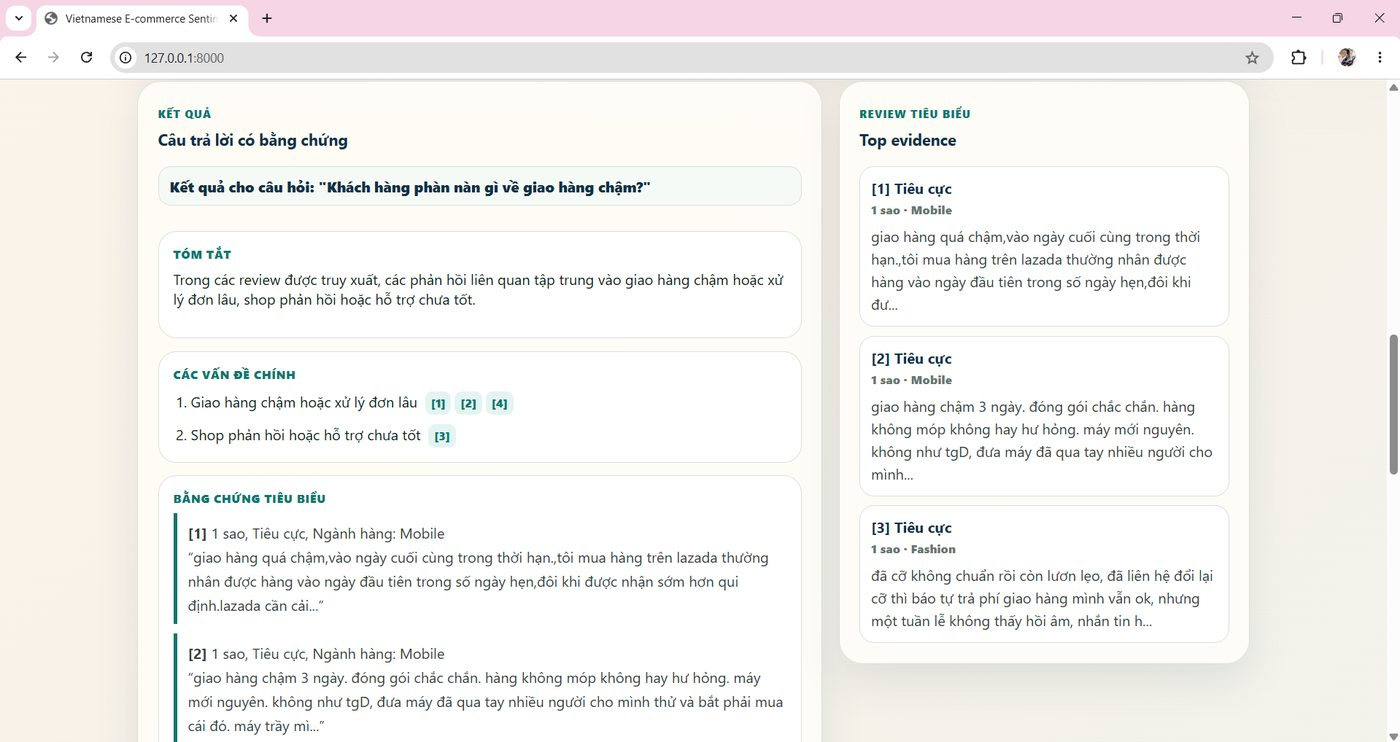
\includegraphics[width=0.92\textwidth]{figures_generated/web_rag_answer_demo.jpg}
    \caption{Kết quả RAG gồm tóm tắt, vấn đề chính, citation và top evidence.}
    \label{fig:web-rag-answer-demo}
\end{figure}

Hình \ref{fig:web-rag-evidence-demo} minh họa vùng review được truy xuất. Mỗi evidence card hiển thị citation id, điểm liên quan, ngành hàng, số sao, sentiment và đoạn review. Các từ khóa liên quan trong review được nhấn mạnh, giúp kiểm tra trực quan vì sao một review được xem là liên quan đến câu hỏi.

\begin{figure}[H]
    \centering
    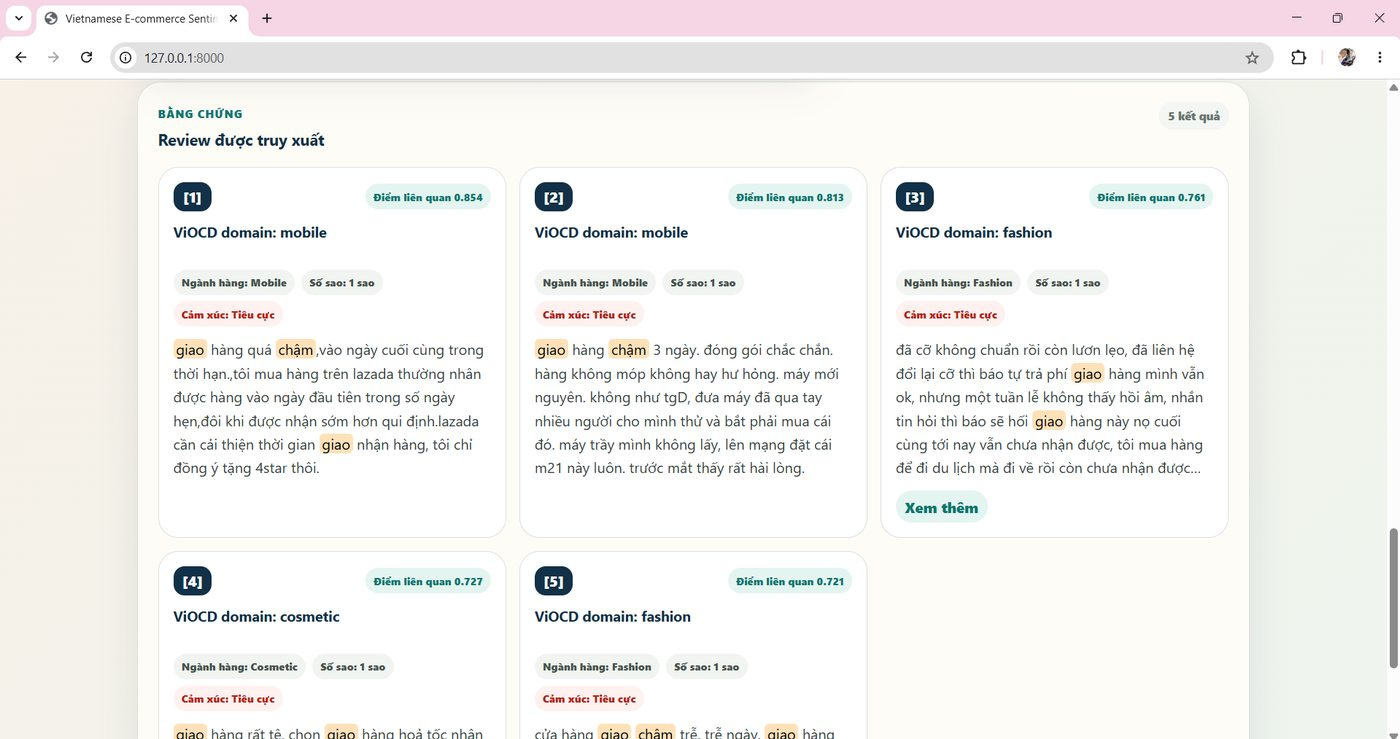
\includegraphics[width=0.92\textwidth]{figures_generated/web_rag_evidence_demo.jpg}
    \caption{Danh sách review được truy xuất trong tab RAG và các evidence cards.}
    \label{fig:web-rag-evidence-demo}
\end{figure}

Hình \ref{fig:web-technical-demo} minh họa tab Kỹ thuật \& đánh giá. Tab này tổng hợp các thông tin quan trọng của bản final như số documents trong kho review, embedding model, retrieval method và baseline Precision@5. Nhờ đó, người đọc có thể đối chiếu nhanh giữa giao diện demo và số liệu đã trình bày trong các chương dữ liệu, phương pháp và thực nghiệm.

\begin{figure}[H]
    \centering
    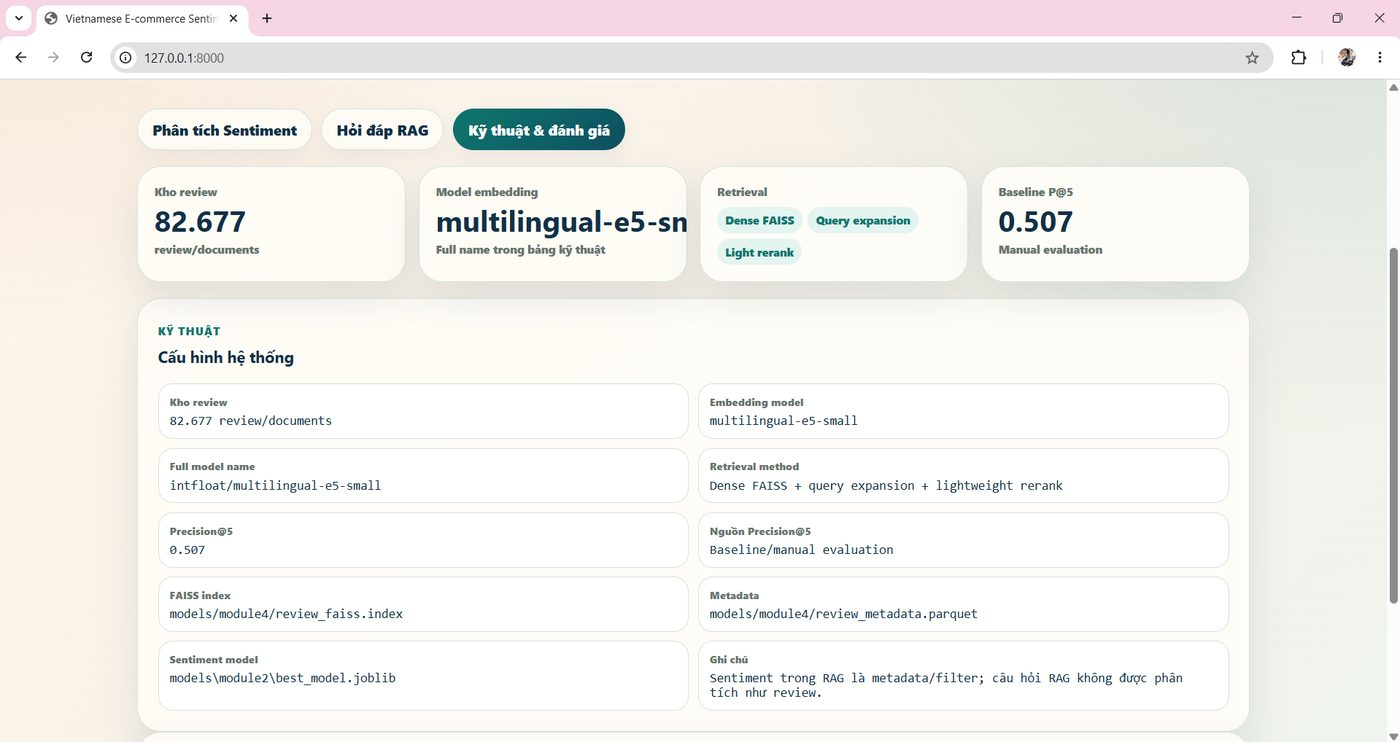
\includegraphics[width=0.92\textwidth]{figures_generated/web_technical_demo.jpg}
    \caption{Tab Kỹ thuật \& đánh giá hiển thị cấu hình hệ thống và metric chính.}
    \label{fig:web-technical-demo}
\end{figure}

\section{Vai trò của giao diện trong kiểm thử hệ thống}
Giao diện giúp kiểm thử tích hợp giữa các artifact và backend. Nếu tab Sentiment trả kết quả, có thể xác nhận artifact sentiment được load đúng. Nếu tab RAG trả answer có citation, có thể xác nhận FAISS index, metadata, embedding model và answer formatter hoạt động cùng nhau. Nếu tab kỹ thuật hiển thị 82.677 documents và embedding model multilingual-E5-small, có thể kiểm tra rằng cấu hình final của Module 4 đang được dùng.

Giao diện cũng hỗ trợ kiểm tra lỗi logic. Ví dụ, khi query thay đổi nhưng chưa chạy lại, UI cần cảnh báo để tránh hiển thị answer cũ như kết quả của query mới. Khi không có evidence đủ mạnh, answer phải trả lời thận trọng. Các kiểm soát này phản ánh nguyên tắc \EvidenceGrounded{} generation của đề tài.

\section{Tóm tắt triển khai}
Tầng triển khai thử nghiệm không làm thay đổi kết quả huấn luyện hoặc FAISS index. Nó đóng vai trò kết nối artifact đã có với người dùng thông qua API và UI. Vì vậy, nếu chỉ chỉnh giao diện hoặc format answer, không cần rebuild FAISS index. Nếu thay corpus, embedding model hoặc cách tạo retrieval text, cần build lại index/metadata và đánh giá lại retrieval.

